\documentclass[11pt,fleqn]{article}
%\usepackage{CJK}
\usepackage{latexsym}
\usepackage{color}
\usepackage{graphicx, float}\usepackage{graphicx}
\usepackage{algorithmic}
\usepackage{algorithm}
%\usepackage{algpseudocode}
%\usepackage[colorlinks]{hyperref}
\usepackage[toc,page]{appendix}
\usepackage{bm}
\setlength{\oddsidemargin}{-0.0in}
\setlength{\evensidemargin}{-0.0in} \setlength{\textwidth}{6.0in}
\setlength{\textheight}{9.0in} \setlength{\topmargin}{-0.2in}
%\usepackage[boxruled]{algorithm2e}

%\setlength{\leftmargin}{0.7in}
\usepackage{amssymb, graphicx, amsmath}  %  fancyheadings,
\usepackage{setspace}
\newcommand\qed{\qquad $\square$}
\newcommand{\nn}{\nonumber}

\def \[{\begin{equation}}
\def \]{\end{equation}}
\def\proof{{\bf Proof:\quad}}
\def \endzm {\quad $\Box$}
\def\dist{\hbox{dist}}


\newcommand{\R}{\mathbb{R}}
%\newtheorem{yinli}{����}[section]
\newcommand{\D}{\displaystyle}
\newcommand{\T}{\textstyle}
\newcommand{\SC}{\scriptstyle}
\newcommand{\FT}{\footnotesize}



%\newtheorem{theorem}{Theorem}[section]
%\renewcommand{\thetheorem}{\arabic{section}.\arabic{theorem}}
\newtheorem{definition}{Definition}
\renewcommand{\thedefinition}{\arabic{section}.\arabic{definition}}
\newtheorem{lemma}{Lemma}[section]
\renewcommand{\thelemma}{\arabic{section}.\arabic{lemma}}
\newtheorem{remark}{Remark}
\renewcommand{\theremark}{\arabic{section}.\arabic{remark}}
\newtheorem{proposition}{Proposition}[section]
\renewcommand{\theproposition}{\arabic{section}.\arabic{proposition}}
\newtheorem{corollary}{Corollary }[section]
\renewcommand{\thecorollary}{\arabic{section}.\arabic{corollary}}
\renewcommand{\theequation}{\arabic{section}.\arabic{equation}}
\renewcommand{\baselinestretch}{1.35}
\newtheorem{exam}{Example}[section]
\renewcommand{\theexam}{\arabic{section}.\arabic{exam}}
\newtheorem{theo}{Theorem}[section]
\renewcommand{\thetheo}{\arabic{section}.\arabic{theo}}
\begin{document}
%\begin{CJK*}{GBK}{song}

\begin{center}

{\LARGE \bf CS391L Machine Learning HW2: Independent Component Analysis}\\

\vskip 25pt
 {Zeyuan Hu, iamzeyuanhu@utexas.edu }\\
\vskip 5pt
{\small EID:zh4378 Fall 2017 }

\end{center}

\begin{spacing}{1.5}
\section{Introduction}

\paragraph{}In this task, we are asked to perform blind source separation by 
applying the Independent Component Analysis (ICA) to sounds data. In details,
suppose there exists an $n$ by $t$ matrix $U$ of $n$ source signals of 
length $t$ and we have an $m$ by $t$ matrix $X$ of $m$ mixed signals
($m\ge n$) of length $t$ that consist of different linear mixtures of $U$,
then, we can recover the original signals $U$ under certain condition.

This writeup is organized in the following way: In the first section, I will 
describe the steps to finish the task. Next, I will talk about the experimentation result. 
Lastly, I will give a breif summary of the whole work.

\section{Method}

\paragraph{}In this section, I will talk about how we work with the raw data, how we perform the ICA on the data, and
how we carry out the experiment. 

\subsection{Work with the data} \label{work with the data}

\paragraph{}In this task, we work with two data files: \verb|sounds.mat| and \verb|icaTest.mat|. The first dataset
contains a varaible called \verb|sounds|, which is $5$ by $44000$ matrix. Each row represents a roughly four
second sound clip and these signals are not mixed. The second dataset contains two matrices: $U$, which is a $3$
by $40$ matrix and $A$, which is $3$ by $3$ matrix. Again, the signals in this dataset is also unmixed. 
The first thing to do is to create the mixed signal matrix $X$. I apply two approaches: for the \verb|sound| matrix,
I randomly create the mixed signal matrix by randomly creating the original signal matrix, and matrix $A$, which
is an $m$ by $n$ matrix such that $A_{i,j}$ is the weight of the $j$th source signal in the ith mixed signal.
The details of the implementation can be found in function \verb|mixSignal| in \verb|hw2.py|. The second approach
is to use the $A$ directly coming from \verb|icaTest.mat| and generate the mixed signal matrix $X$ with $X = AU$
using the $U$ from \verb|icaTest.mat| as well. One important step is to convert the datatype of
all the matrices into \verb|float32| in Python, which allows us to keep precision when we do the calculation.

\subsection{Algorithm Implementation}

\paragraph{}In order to uncover the original signals from the mixed signals, we assume
that there is no correlation between source signals and so any correlation between 
different mixed signals is due to a common signal showing through the mixture. Then, our task
is to find a matrix $W$ that recovers the original $n$ source signals 
(possibly in a different order and with different scale factors). In this project, I use 
gradient descent method to decrease the mutual information between signals and thus cover
the original signals:

\begin{enumerate}
\item Assume $X = AU$.
\item Initialize the ($n$ by $m$) matrix $W$ with small random values.
\item Calculate $Y = WX$.
\item $Y$ is our current estimate of the source signals.
\item Calculate $Z$ where $z_{i,j} = g(y_{i,j}) = 1/(1+e^{-y_{i,j}})$ 
for $i \in [1 \dots n]$ and $j \in [1 \dots t]$ (where $t$ is the length of the signals).
This helps us traverse the gradient of maximum information separation.
\item Find $\Delta W = \eta(I + (1-2Z)Y^T)W$ where $\eta$ is a small learning rate.
\item Update $W = W + \delta W$ and repeat from step 3 until convergence or some max iterations reached.
\end{enumerate}

The implementation of the algorithm can be found in function \verb|ica|. There are a couple of implementation
details need to notice:

\begin{itemize}
\item We use uniform distribution between 0 and 1 to generate the initial weights $W$.
\item I setup a threshold value $H$, which equals to $1\times10^{-9}$. Let our unmixing matrix
in $i$-th iteration be $W_i$. Let the norm of difference of unmixing matrices in two neighbor
iterations be $\Delta$. Then, in addition to the max iterations termination condition, the 
algorithm can also stop when $\Delta < H$. In the implementation, I set the max iterations to 
$1000000$ and the algorithm usually stops at around $6000$ iterations.
\item The learning rate $\eta$ I set in the implementation is $0.01$. After several experimentations,
I find this learning rate gives the best result in the recovered signals.
\end{itemize}

\section{Results}

\paragraph{}I run the ICA algorithms on both \verb|icaTest.mat| and \verb|sounds.mat| datasets and plot
the original signals,  the mixed signals, and the recovered signals.

\subsection{IcaTest.mat}

\paragraph{}Once we implement our algorithm, we want to verify if it works on a small set of data. 
As described in the section \ref{work with the data}, \verb|icaTest.mat| is the ideal candidate
for this purpose. The figure 1 is what I get after running ICA algorithm on this dataset:

\begin{figure}
\centering
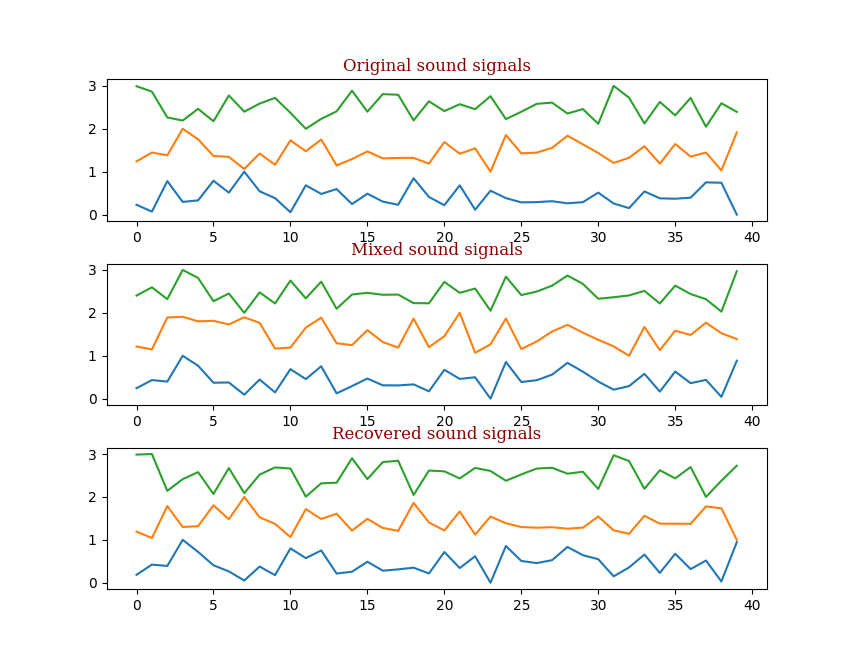
\includegraphics[scale=0.6]{icaTest.png} 
\caption{ICA on icaTest.mat}
\end{figure}

The result heavily relies on the learning rate $\eta$ and the number of iterations we perform the gradient
descent. In this experiment I find out that once the $\Delta$ belows the threshold value $H$, there is not
much gain from performing extra iterations of gradient descent.

\subsection{Sounds.mat}

\paragraph{} \verb|sounds.mat| offers an opportunity for us to test out our ICA algorithm in a "big data"
setting and the result is quite good for my implementations. Figures 2-6 show the plot of 
the original signals,  the mixed signals, and the recovered signals under the different kind of mixture.

\begin{figure}
\centering
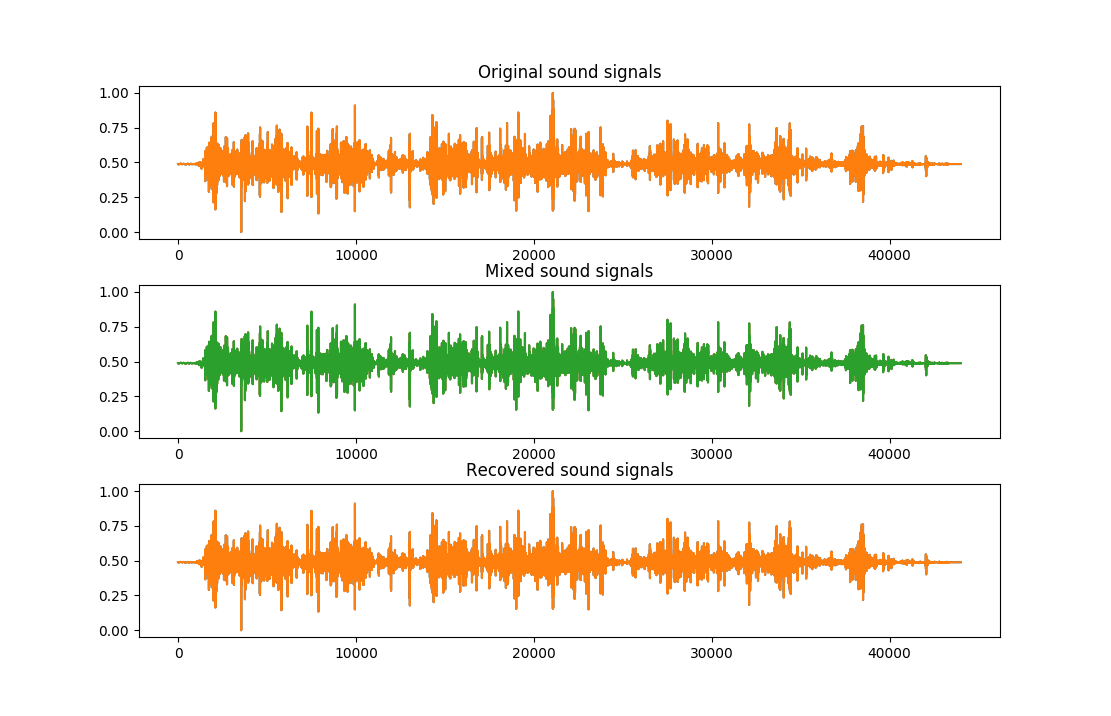
\includegraphics[scale=0.6]{sounds01.png} 
\end{figure}

\begin{figure}
\centering
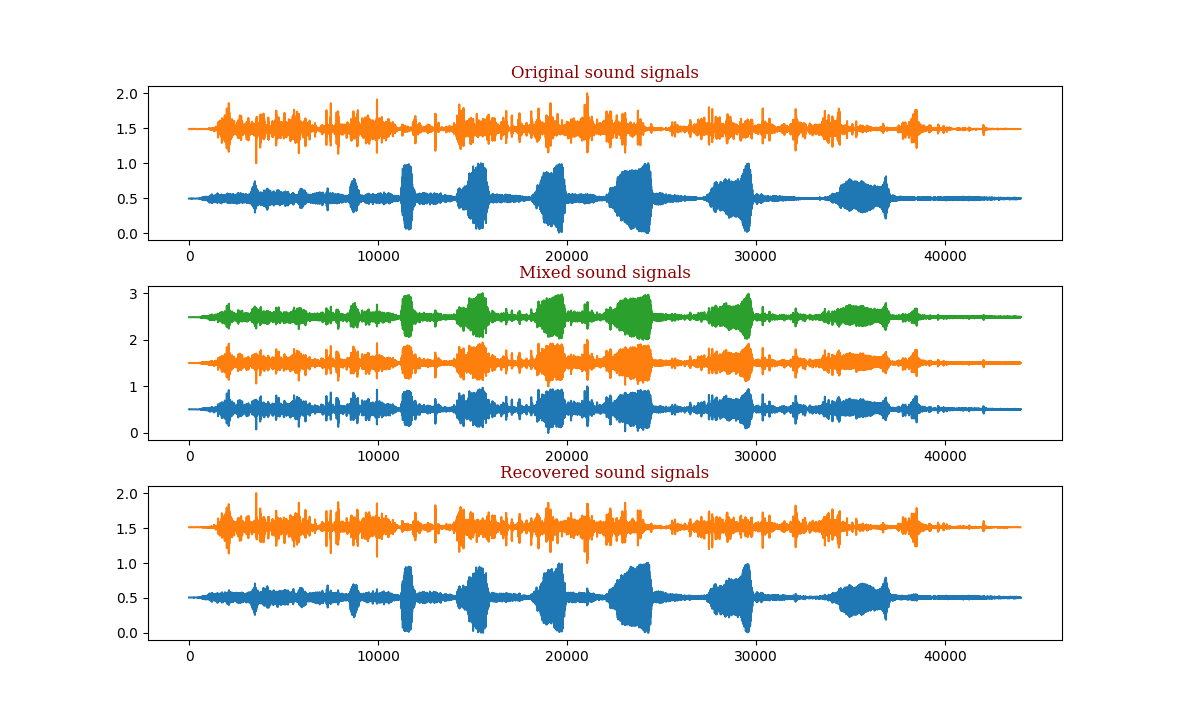
\includegraphics[scale=0.6]{sounds02.png} 
\end{figure}

\begin{figure}
\centering
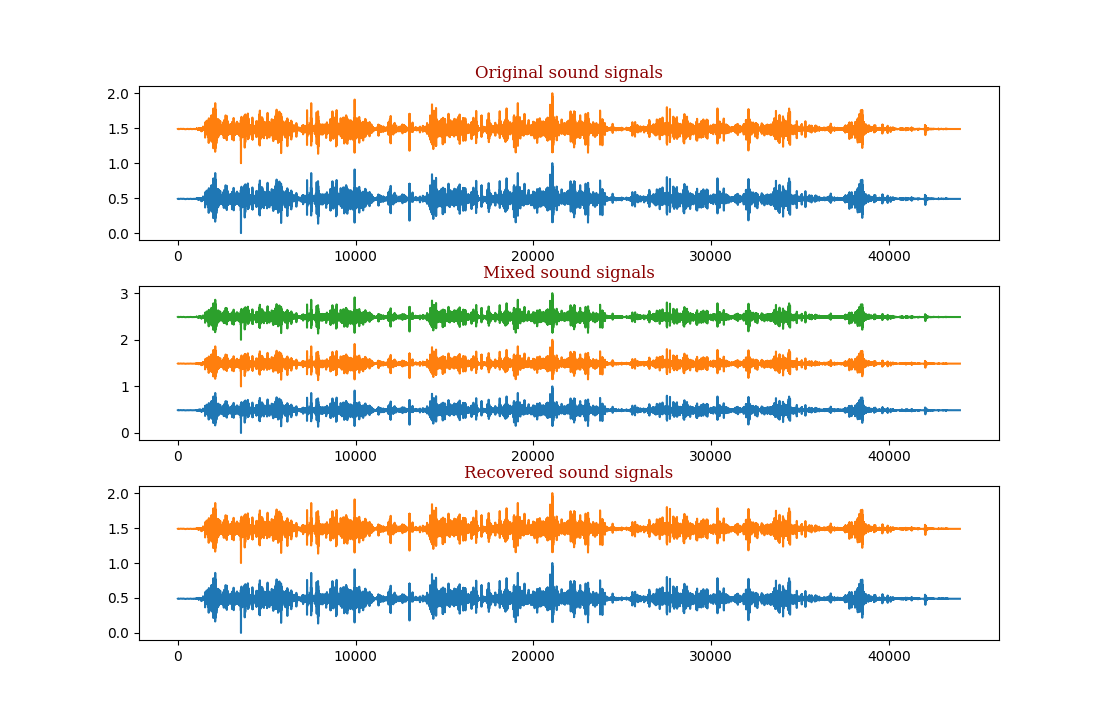
\includegraphics[scale=0.6]{sounds03.png} 
\end{figure}

\begin{figure}
\centering
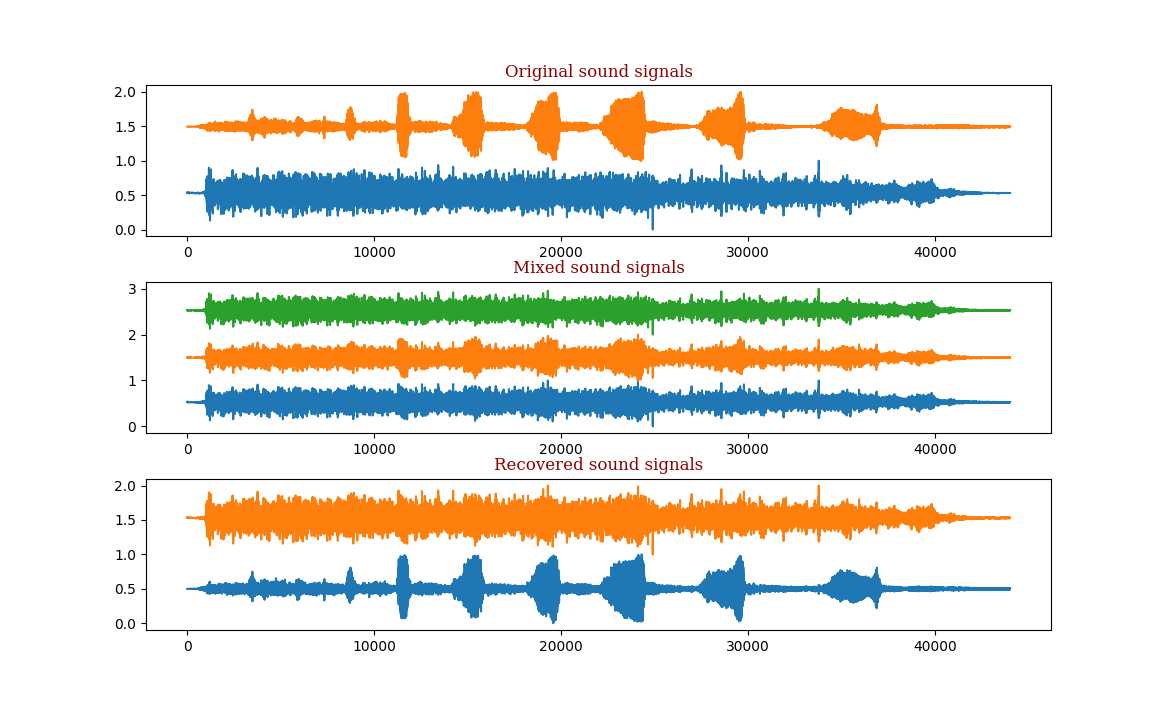
\includegraphics[scale=0.6]{sounds06.png} 
\end{figure}


\section{Summary}

\paragraph{}In this task, I apply ICA method to sound data to perform blind source separation. 
I perform the algorithm using different size of data and find out the performance of the 
algorithm is quite good under the both situations. In addition, I tune the learning rate,
the number of iterations, and the threshold value in the gradient descent in order to get
the best performance of the algorithm.

\end{spacing}

\begin{appendices}

\section{How to run the code}

\paragraph{}To run my code, unzip the \verb|hw2.zip| and put the data file \verb|sounds.mat| and \verb|icaTest.mat| 
under the same directory with \verb|hw2.py|. Then, you
can run the code with the command \verb|python3 hw2.py ICATEST| or \verb|python3 hw2.py SOUNDS|. 
The former command applies ICA towards \verb|icaTest.mat| dataset and the latter command applies
ICA towards \verb|sounds.mat| dataset. The output of both commands will be the plot of 
the original signals,  the mixed signals, and the recovered signals.
My code is heavily commented and please take a look if there are any type of questions.

\end{appendices}

%\end{CJK*}
\end{document}
